\documentclass[11pt, a4paper]{article}
\usepackage{graphicx} % Required for inserting images
\usepackage[T2A]{fontenc}
\usepackage[utf8]{inputenc}
\usepackage[russian]{babel}
\usepackage{amsmath, amssymb}
\usepackage[usenames]{color}
\usepackage{colortbl}
\usepackage{animate}
\usepackage{fancyhdr}
\usepackage{enumitem}
\usepackage{titlesec}
\usepackage{multicol}
\usepackage[backend=biber, style=authoryear]{biblatex}
\addbibresource{source.bib}
\usepackage{csquotes}


\usepackage{geometry}
\geometry{
  a4paper,
  top=30mm, 
  right=5mm, 
  bottom=20mm, 
  left=5mm,
  headheight=50pt
}


\newcommand{\mydate}{Декабрь, 2025}
\newcommand{\myauthor}{В. Алексеев, Д. Малеева, Н. Гончар}

\fancyhf{}
\fancyhead[L]{\large \textit{Научная студия 2025. Переменные звезды. Финальный отчет.}}
\pagestyle{fancy}

\fancypagestyle{firstpage}{
  \fancyhf{}
  \fancyhead[L]{\hspace{-15pt}
\includegraphics[width=0.3\linewidth]{ЦУ.png}}
  \fancyhead[R]{\mydate\\\textit{\myauthor}\\}
}

\begin{document}
\thispagestyle{firstpage}

\noindent
\hspace*{0.5cm}
\begin{minipage}{0.8\textwidth}
\LARGE \textbf{Применение методов машинного обучения для поиска и классификации переменных звезд}
\end{minipage}\vspace{20pt}

\hspace{0.2\textwidth}\begin{minipage}{0.7\textwidth}
\section*{Аннотация}
Непрерывно развивающиеся системы сбора астрономических данных (космические телескопы, крупные наземные обсерватории) ежедневно дополняют и обновляют каталоги миллионами записей, которые необходимо обрабатывать с тем же темпом. Используя каталог APASS, мы выявили цветовые индексы из данных фотометрии и обучили на них бинарный и мультикассовый классификатор. В итоге мы получили модели с достаточно высоким f1-score $\approx 96\%$ для бинарной классификации и accuracy $\approx 60\%$ для мультиклассовой.
\end{minipage}

\begin{multicols}{2}
\section{Введение}
Астрономические данные возросли в темпе появления, и соответственно, количестве. Основанная причина этого -- новое поколение телескопов, которые уже давно  не только делают обычные снимки звездного пространства, но и собирают фотометрические данные: видимый диапазон, ультрафиолетовый, рентгеновский, инфракрасный, отслеживают изменения в магнитуде объекта со временем, накопленные ошибки измерений -- для миллионов объектов ежедневно. Обрабатывать такую информацию как раньше уже не представляется возможным, в связи с этим в 2011 вышла статья \autocite{first-article}, в которых впервые в задаче для поиска переменных звезд использовались методы машинного обучения. За последние 10 лет таких статей вышло уже десятки и в них сформировался определенный шаблон: исследование параметров набора данных, исключение статистически не значимых признаков, обучение нескольких моделей, оценка результата, выбор наилучшей модели, стекинг с использованием различного рода boosting-моделей (XMLGbooster, CatBooster, GradientBooster, и пр.), окончательный результат и подведение итогов. 

В статье \autocite{Hosenie2019} описывается подход, использующий минимальное кол-во признаков (в основном статистические параметры данных фотометрии), который сумел показал высокий результат (accuracy $\approx 99\%$), однако данный результат достигается лишь в случае классификации двух типов переменных звезд $\delta$-щита и ACEP (Anomalous
Cepheids), общее значение accuracy оказалось на уровне $\approx 61\%$. Данное исследование опиралось на идею о том, что использование чрезмерного количества признаков не улучшает, а зачастую ухудшает показатели модели.

В этой статье мы представим наш взгляд на проблему поиска переменных звезд и одно из возможных решений. 

\section{Данные}
Окончательный набор данных состоит из пересечения трех обзоров:
\begin{itemize}
    \item[i)] APASS (AAVSO Photometric All-Sky Survey) -- астрономический фотометрический опрос, целью которого является измерение оптических (например, $V$ и $B$) величин для миллионов звёзд по всему небу. Данные APASS используются для калибровки изображений, исследования яркостных изменений и определения фотометрических характеристик объектов. Фотометрия APASS имеет высокую точность для звезд с диапазоном яркости примерно от 10 до 17 магнитуд.
    \item[ii)] GALEX (Galaxy Evolution Explorer) -- это космический телескоп, который проводил ультрафиолетовый (УФ) обзор неба. Данные GALEX включают измерения в двух УФ диапазонах: $FUV$ (фундаментально коротковолновой УФ) и $NUV$ (ближний УФ). Эти данные особенно полезны для исследования молодых звёзд, переменных объектов с УФ-излучением, а также для изучения процессов звёздного формирования и эволюции галактик.
    \item[iii)] 2MASS (Two Micron All-Sky Survey) -- это всенебесный фотометрический обзор, выполненный в ближнем инфракрасном диапазоне. Он обеспечивает измерения в трёх стандартных инфракрасных фильтрах: $J$ (1.25 мкм), $H$ (1.65 мкм), $K_s$ (2.17 мкм). Данные 2MASS используются для изучения структуры Млечного Пути, исследования звёздных скоплений, выявления объектов, скрытых межзвёздной пылью, и для анализа галактик.
\end{itemize}
В конечном итоге, имеем объединенный набор данных, содержащий информацию о фотометрии объектов практически во всех диапазонах, а также период изменения светимости объекта (если таковой обнаружен). Это дает возможность составить всевозможные цветовые индексы, что крайне важно для выявления типа переменной звезды \autocite{first-article}. Полный список признаков приведен в табл. ~\ref{tab:datasetinfo}.

Общее количество записей (до обработки) -- $56\;298$, среди них переменных -- $5\;910$, что составляет $\approx10,5\%$ от всего набора. Всего уникальных типов переменных звезд -- 111. Наиболее частые: ротационные, $\delta$-щита, $SX$ феникса и Гамма Дораду. Мы не станем, в отличие от \autocite{Hosenie2019}, исключать некоторые виды переменных звезд, чтобы не ограничивать общность данного исследования.

\section{Генерация признаков (features)}
Данные сильно перемешаны, поэтому использование значений фотометрии напрямую как признака для модели повлечет за собой плохую точность и, в контексте деревьев, переобучение. Поэтому было принято решение перейти от точечных данных к линейным комбинациям, т.е. цветовым индексам. Мы сгенерировали их как всевозможные неупорядоченные попарные разности, тем самым не потеряв информацию об объекте.

Однако искомый набор данных продолжает сохранять сильное наложение классов, как для бинарной классификации, так и для многоклассовой (рис.~\ref{fig:tsne}).

Кроме того, из диаграмм распределения t-SNE видно, что для обоих случаев классификации имеет место сильный дисбаланс классов, численно это было описано в  п. 2.
\begin{figure*}
    \centering
    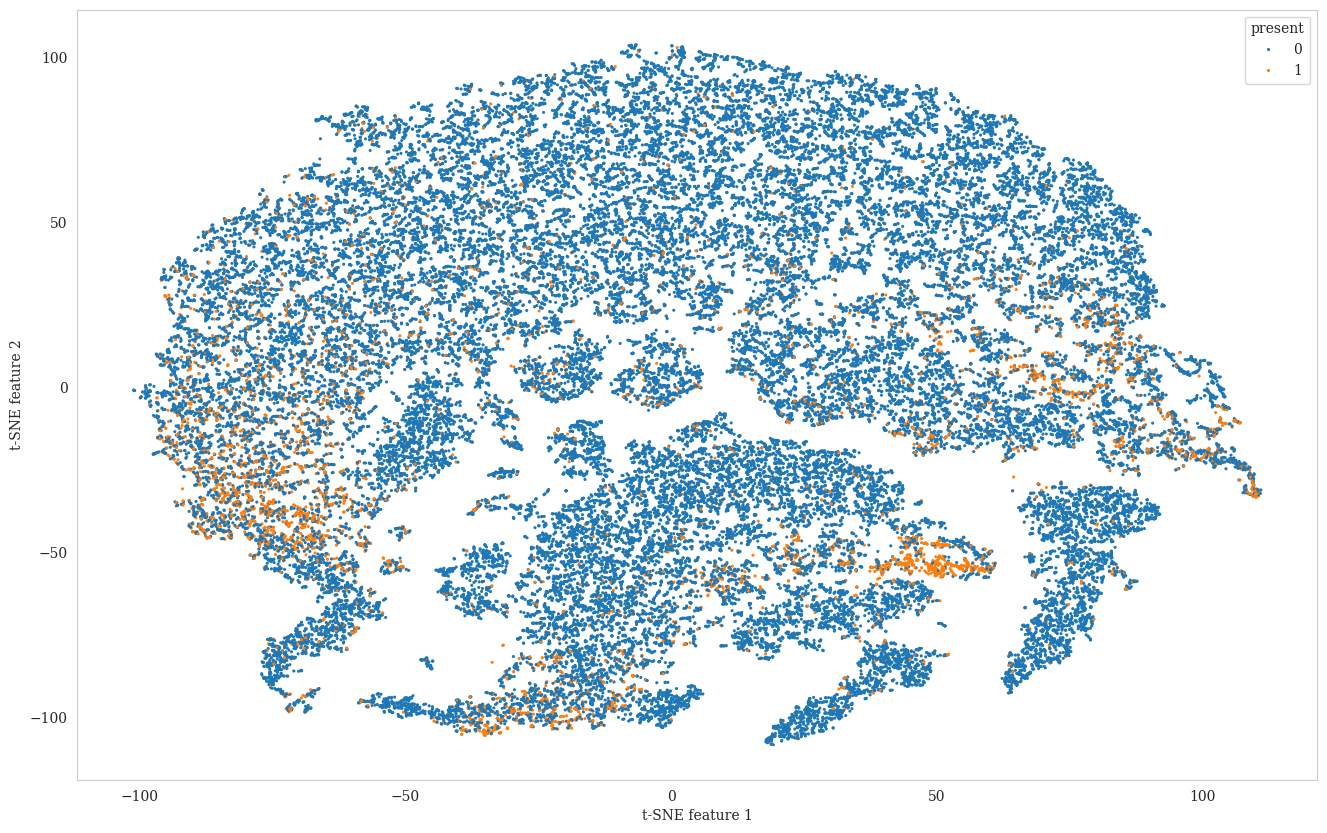
\includegraphics[width=0.45\linewidth]{tsne (binary).png}
    \hspace{12pt}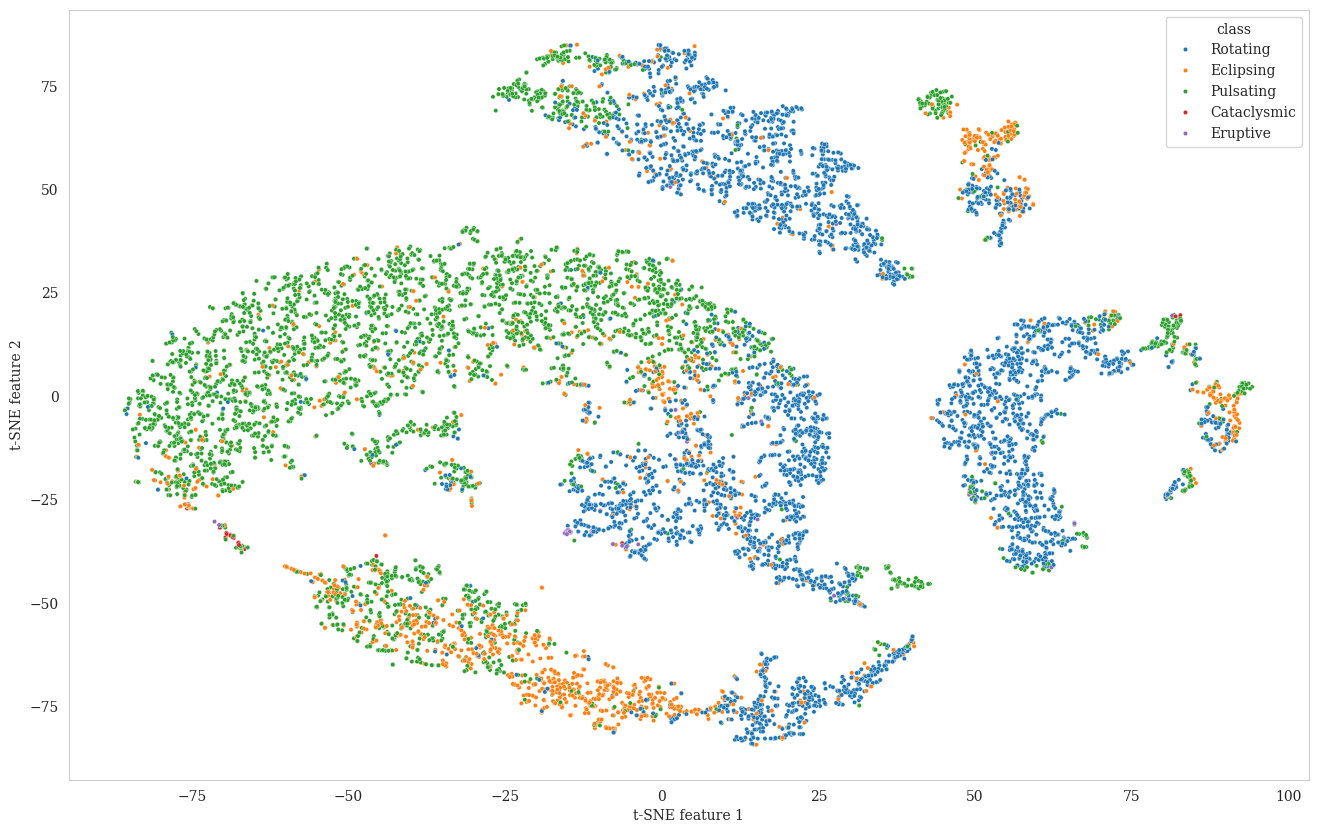
\includegraphics[width=0.45\linewidth]{tsne (multiclass).png}
    \caption{t-SNE проекция набора данных}
    \label{fig:tsne}
\end{figure*}
\section{Алгоритм классификации}
\subsection{Бинарная классификация}
Исходя из предпосылок, описанных в предыдущем параграфе, в качестве базового классификатора не имеет смысла брать линейные модели (такие как Linear Regression, SVM) помимо этого, наиболее часто используемый метод k ближайших соседей (kNN) также не покажет должного уровня эффективности, поскольку данные распределены далеко не равномерно: их размах достаточно большой, притом распределение близко к нормальному.

В таких случаях применяется другой, не менее популярный метод машинного обучения -- деревья решений (DT -- \textit{от англ. Deсision Tree}). Данная модель делает выбор на основе коэффициента Джини (Gini impurity) или коэффициента полученной информации (Information Gain):
\begin{gather}G=\sum_{i=1}^C p_i^2, \text{ доля $i$-го класса в узле.}\\
\Delta G=G_{parent} -\frac{N_{left}}{N}G_{left}-\frac{N_{rgiht}}{N}G_{right}
\end{gather}
Алгоритм фиксирует $j$-й класс и максимизуерт величину выигрыша $\Delta G$ для него. Он устойчив к описанному состоянию набора данных, однако имеет существенный минус -- переобучение. Классическим, в данном контексте, решением приводится горизонтальное масштабирование модели, в частности, они образуют альянс деревьев решений. В нашем исследовании мы будем использовать одну из возможных реализаций -- Random Forest Classifier.

Вообще говоря, указанная модель является самой частой по упоминанию в исследованиях на тему поиска переменных звезд после упоминания ее в \autocite{Bloemen2001}.
\begin{figure*}
    \centering
    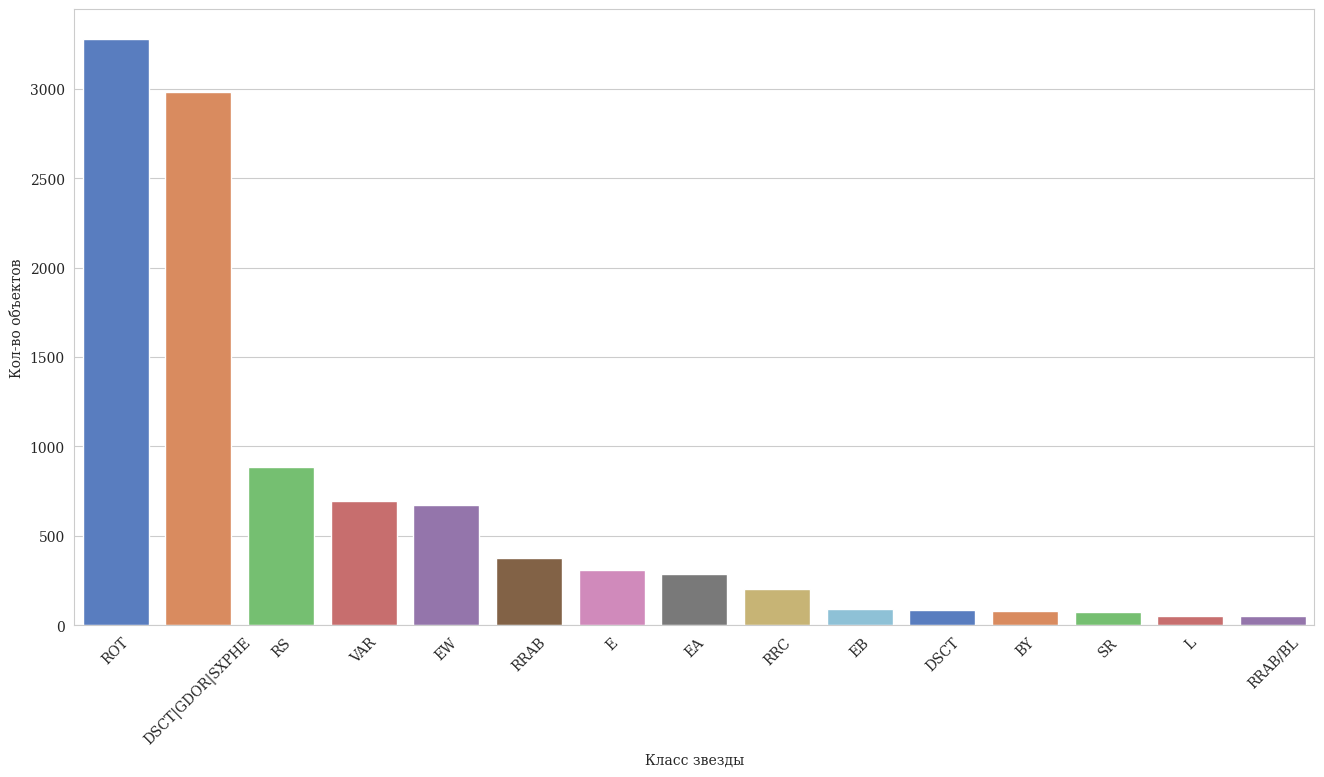
\includegraphics[width=0.75\linewidth]{histmulti.png}
    \caption{Диаграмма распределения исходных классов (15 самых крупных)}
    \label{fig:histmulti}
\end{figure*}
\subsection{Многоклассовая классификация}
Для мультиклассовой классификации верны те же утверждения, что и для бинарной, однако ситуацию усугубляет большее кол-во классов ($C\approx 100$), поэтому точность модели неизбежно падает.

Тем не менее есть способ, позволяющий кратно увеличить показатели: укрупение указанных классов. Диаграмма распределения исходных приведена на рис. ~\ref{fig:histmulti}. В качестве решения мы предлагаем использовать укрупненную схему классов, основанную на сходстве физических свойств исходных, в частности:
\begin{enumerate}
    \item \textit{Эруптивные} -- эти звёзды демонстрируют вспышки, выбросы массы или нерегулярные яркостные всплески. У них нет стабильного периода, всё происходит хаотично, зачастую достаточно редко. Процессы носят взрывной или квазивзрывной характер (напоминает взрыв, но в строгом смысле слова им не является) и часто связаны с нарушением гидростатического равновесия. Подавляющее большинство таких звезд находятся на ранних стадиях эволюции, на поздних реже. Их изменчивость вызвана мощными выбросами вещества и энергии, причиной могут служить аккреция (процесс накопления массы извне на поверхности), магнитные пересоединения (взрывное преобразование энергии магнитного поля в тепло и кинетическую энергию частиц), сброс оболочки из-за светового давления, неустойчивое горение. 
    
    \item \textit{Пульсирующие} -- их переменность регулярна и обусловлена ритмичными расширениями и сжатиями самой звезды. Причиной являются внутренние термодинамические процессы, как правило процесс зарождается в зоне ионизации гелия (иногда водорода). При сжатии газ в этой зоне ионизируется, становится более непрозрачным, задерживает излучение, давление растёт и звезда расширяется. При расширении газ остывает, рекомбинирует, прозрачность растёт, давление падает – звезда сжимается под действием гравитации. Далее цикл повторяется. Пульсирующие звёзды могут быть самых разных масс и стадий эволюции. 
    
    \item \textit{Ротационные} -- звезды, чья переменность блеска вызвана их вращением. Изменения связаны с неоднородностью поверхности и осевым вращением звезды она, будто «подставляет» под обзор разные части поверхности, яркость которой может быть неодинакова по всей площади, например, из-за скопления определенных химических элементов в одной части или же из-за эффекта Доплера, при быстром вращении и сплюснутости (она сама по себе так же может являться причиной ротационной переменности).
    
    \item \textit{Катаклизмические} – системы с резкими всплесками яркости. Фактически подкласс эруптивных, характеризующийся чаще всего взрывными действиями в тесных двойных системах на поздних стадиях эволюции (например, в системах, где белый карлик аккрецирует вещество со звезды-компаньона, обычно красного карлика или субгиганта). 
    
    \item \textit{Затменные} -- вероятно, самые распространённый вид переменности. Падение блеска вызвано не внутренними химическими и физическими процессами, а геометрическим покрытием одного компонента системы другим при их орбитальном движении относительно луча зрения наблюдателя. То есть если посмотреть на систему под другим углом, переменность может исчезнуть.
    
    \item \textit{Рентгеновские} -- звёзды, переменность которых наблюдается не в оптическом диапазоне, а в рентгеновском, в нём демонстрируются значительные изменения со временем. Почти всегда это свидетельствует о наличии компактного объекта в тесной двойной системе, аккрецирующего на себя вещество со второй звезды. Если это вещество падает с очень высокой скоростью, оно разогревается до температур жёсткого рентгеновского диапазона. Изменения в темпе аккреции из-за сложных процессов в аккреционном диске и на поверхности компактного объекта как раз являются причиной переменности.
    
    \item \textit{Уникальные} -- непериодические переменные, не имеющие аналогов в стандартных классах. У них сложное, неповторимое поведение. Причиной может быть уникальное, может единичное событие в процессе жизни звезды, механизм которого еще недостаточно описан.
    \end{enumerate}

    \section{Обучение модели. Оценка результатов}
    Далее мы использовали стандартное обучение с учителем, т.е. передали модели описанный выше набор данных, после чего оценили результаты по следующим метрикам: f1-score, balanced accuracy, recall и precision.

    \subsection{Результаты бинарной классификации}
    Результаты моделей классификации наиболее информативно представлять в виде матрицы ошибок (Confusion Matrix), представлена на рис. ~\ref{fig:cmb}.

    Также обращаем внимание на таблицу с полученными метриками:
    \begin{center}
    \renewcommand{\arraystretch}{1.25}
        \begin{tabular}{lccc}
        \hline\hline
            Type & precision & recall & f1-score \\ \hline
            non-Variable & 0.98 & 0.83 & 0.90 \\
            Vairable & 0.37 & 0.85 & 0.51 \\
        \hline\hline
    \end{tabular}
    \end{center}
    Проделанная работа демонстрирует хорошие результаты в сравнении с наивной моделью Байеса \autocite{Wozniak2003}. Кроме того стоит обратить внимание на на достаточно высокий показатель balanced accuracy $\approx84\%$ и precision $\approx 92\%$ (агрегированный, с учетом количества объектов классов). В контексте поставленной задаче важно именно это значение, поскольку условие \textit{не пропустить} потенциальный переменный объект имеет больший приоритет.

    \subsection{Результаты мультиклассовой классификации}
    Матрица ошибок и основные метрики представлены на рис. ~\ref{fig:cmb} и в таблице ниже:
    \begin{center}
    \renewcommand{\arraystretch}{1.25}
    \begin{tabular}{lccc}
        \hline\hline
            Type & precision & recall & f1-score \\ \hline
            Cataclysmic & 0.05 & 0.50 & 0.10 \\
            Eclipsing & 0.32 & 0.40 & 0.36 \\
            Eruptive & 0.05 & 0.60 & 0.09 \\
            Pulsating & 0.85 & 0.74 & 0.79 \\
            Rotating & 0.87 & 0.75 & 0.80 \\
        \hline\hline
    \end{tabular}
    \end{center}
    Из матрицы сразу выявляется три типа ошибок модели: i) пульсирующие и затменные ii) ротационные и затменные iii) ротационные и эруптивные. Более глубокий анализ природы этих ошибок показал, что в каждом из случаев происходит сильное вмешивание по всем параметрам (период, данные фотометрии), однако наблюдаемое верно не для всех звезд класса, а лишь для части. Вследствие чего мы сделали вывод, что наша модель разбиения не является наилучшей. Далее мы подробно опишем, какие факторы стоило учесть, чтобы получить лучшие метрики.

    Заметим также, что общая точность составляет $\approx69 \%$, что является достаточно неплохим показателем для мультиклассовой классификации ($N_{classes}=5$) с сильным дисбалансом классов.
\end{multicols}
\begin{table}
    \centering
    \renewcommand{\arraystretch}{1.5}
    \begin{tabular}{lr}
        \hline\hline
        RAJ2000, DEJ2000 & координаты звезд\\
        $N_{obs}$ & количество наблюдений\\
        $V$, $B$, $g$, $rp$, $ip$, $FUV$, $NUB$, $J$, $H$, $K$ & данные фотометрии\\
        $V_{err}$, $B_{err}$, ..., $K_{err}$ & ошибки измерений \\ 
        present & индикатор переменности звезды \\
        type & детальное обозначение типа переменной звезды \\
        $T$ & период изменения светимости \\ \hline
        \hline
    \end{tabular}
    \caption{Список признаков используемого набора данных}
    \label{tab:datasetinfo}
\end{table}
\begin{figure}
    \centering
    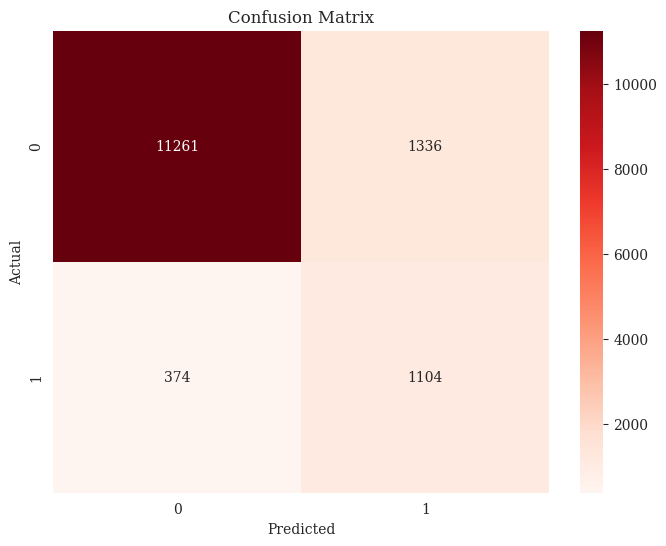
\includegraphics[width=0.45\linewidth]{cmb.png}
    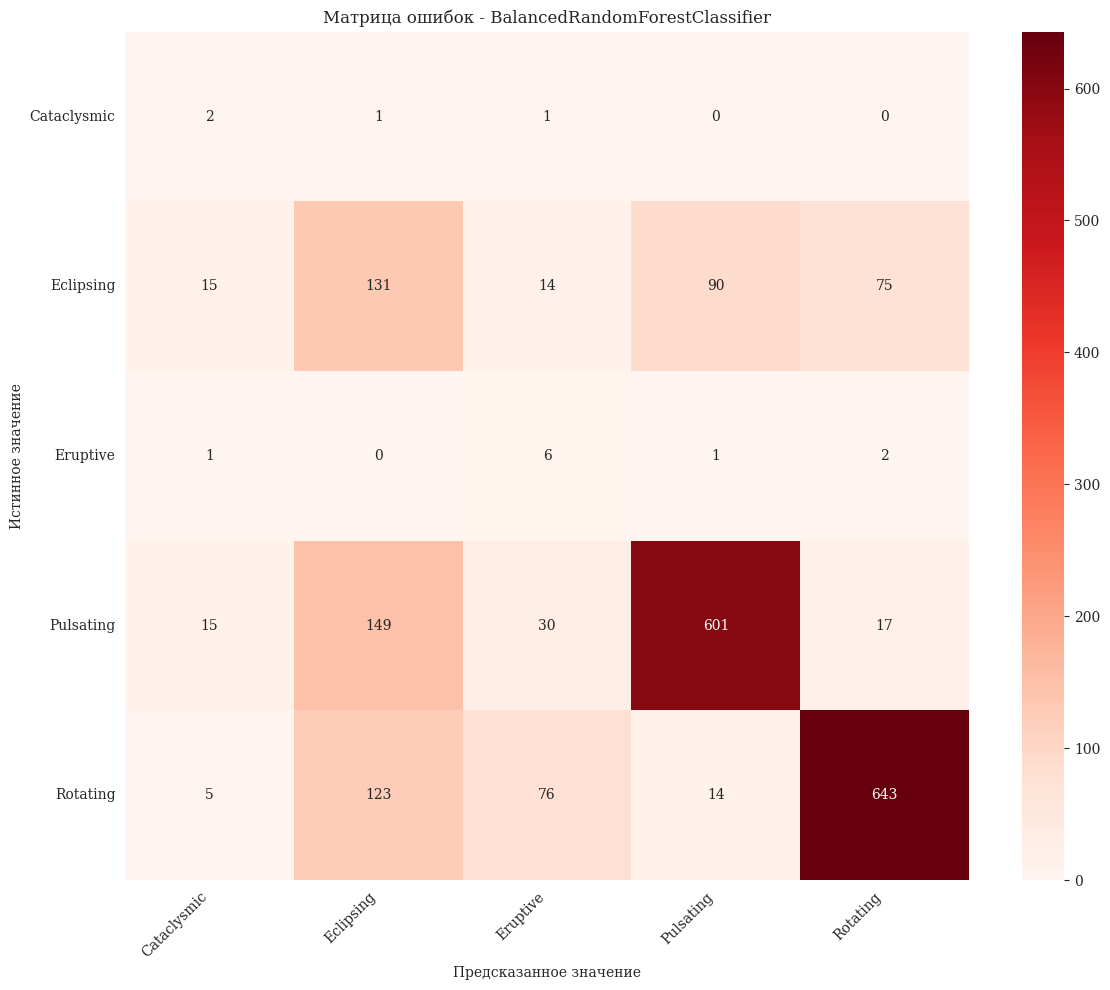
\includegraphics[width=0.45\linewidth]{cmm.png}
    \caption{Матрица ошибок классификации}
    
    \label{fig:cmb}
\end{figure}

\begin{multicols}{2}
    \section{Дальнейшие шаги}
    \subsection{Улучшение модели}
    Улучшить имеющиеся показатели можно не прибегая к пересмотру изначальной физической задачи. Использование различного рода бустингов (Linear Boosting, Cat Boosting, XML Boosting) в зависимости от случая могут дать прирост до $10\%$ в f1-score'е. Кроме того имеет смысл провести аудит среди других методов машинного обучения. Наиболее перспективный на наш взгяд -- генетическое обучение. Подобный подход уже был применен в статье \autocite{Bloom2011}, однако в ней упоминалось множество возможных улучшений, которые заинтересовали нас.
    
    \subsection{Пересмотр схемы укрупнения}
    Касательно многоклассовой классификации, следует глобально пересмотреть схему укрупнения классов. Из полученных метрик мы ясно выявили, что текущее разбиение не позволяет точно определить принадлежность смежных классов к конкретному, следовательно, логично минимизировать число возможных пересечений в некоторой улучшенной схеме.

    \section{Заключение}
    Методы машинного обучения,  в частности Random Forest, имеют место в астрономии, в поиске переменных звезд, впоследствии их классификации. На данный момент мы не смогли получили модель, способную заменить астрономов по точности, однако сумели обогнать их по скорости. В перспективе, машинное обучение точно сумеет занять эту нишу. 

    \section{Приложение}
    \subsection{Формулы расчета метрик}
    Точность:
    $$\text{accuracy}=\frac{TP}{TP+TN+FP+FN}$$
    Чистота:
    $$\text{precision}=\frac{TP}{TP+FP}$$
    Полнота:
    $$\text{recall} =\frac{TP}{TP+FN}$$
    Метрика f1:
    $$\text{f1-score} =2\cdot\frac{\text{Precision}\cdot \text{Recall}}{\text{Precision}  + \text{Recall}}=\frac{2TP}{2TP+FP+FN}$$
    Сбалансированная точность:
    $$\text{balanced accuracy}=\frac{1}{n}\left(\frac{TP}{TP+FN}+\frac{TN}{TN+FP}\right)$$
    \subsection{Ссылки}
    \printbibliography
\end{multicols}

\begin{minipage}{0.7\textwidth}
\begin{quote}
    \textit{If I have seen further it is by standing on the shoulders of Giants.} -- Исаак Ньютон.
\end{quote}
\end{minipage}
\end{document}
